\section{Trusted Execution Environments}
Trusted Execution Environments (TEEs) are isolated computing environments that provide strong security guarantees for code and data execution, even in the presence of potentially compromised operating systems and applications. They achieve this by leveraging hardware-based isolation mechanisms to establish secure boundaries, often called enclaves, where sensitive computation can occur without interference from the rest of the system. TEEs aim to ensure confidentiality and integrity through careful hardware and software co-design, minimizing the trusted computing base (TCB) and mitigating a wide range of software attacks. While several commercial TEEs, such as Intel Software Guard Extensions (SGX) and ARM TrustZone, demonstrate the feasibility and practical relevance of enclave-based secure execution, their closed-source and inflexible designs limit research and hardware/software co-design opportunities. This has motivated the development of open TEE frameworks like Keystone, built on RISC-V—an open and extensible instruction set architecture. A key architectural feature of TEEs is privilege separation, where a minimal TCB executes in a highly privileged mode controlling access to critical physical resources, while the operating system and applications run in less privileged, untrusted modes.

\section{Keystone architecture overview}

Keystone represents an open-source framework designed to facilitate the architecture and implementation of Trusted Execution Environments (TEEs) leveraging hardware enclaves on RISC-V processors. Its primary objective is to enable the construction of customizable TEEs optimized for specific RISC-V platforms, thereby achieving enhanced performance, reduced trusted computing base (TCB) complexity, and improved programmability tailored to distinct workloads and security threat models.

A typical Keystone-capable system architecture comprises multiple components distributed across different privilege modes of the RISC-V privilege hierarchy. The foundational hardware is a trusted CPU package integrating Keystone-compatible RISC-V cores and a silicon root of trust, potentially augmented by features such as cache partitioning, memory encryption, and secure randomness sources. The core security functionality is governed by the Security Monitor (SM), a minimalistic M-mode software component embodying the system's TCB. The SM is responsible for enclave lifecycle management and enforces isolation boundaries between enclaves and the untrusted operating system (OS).

Keystone’s Security Monitor (SM), executing at the highest privilege level (M-mode), serves as the linchpin of the system’s trusted computing base. Beyond enclave lifecycle management, the SM enforces fine-grained memory isolation policies and orchestrates enclave scheduling, maintaining strict control over resource access to prevent unauthorized interference.

\begin{figure}[htbp]
    \centering
    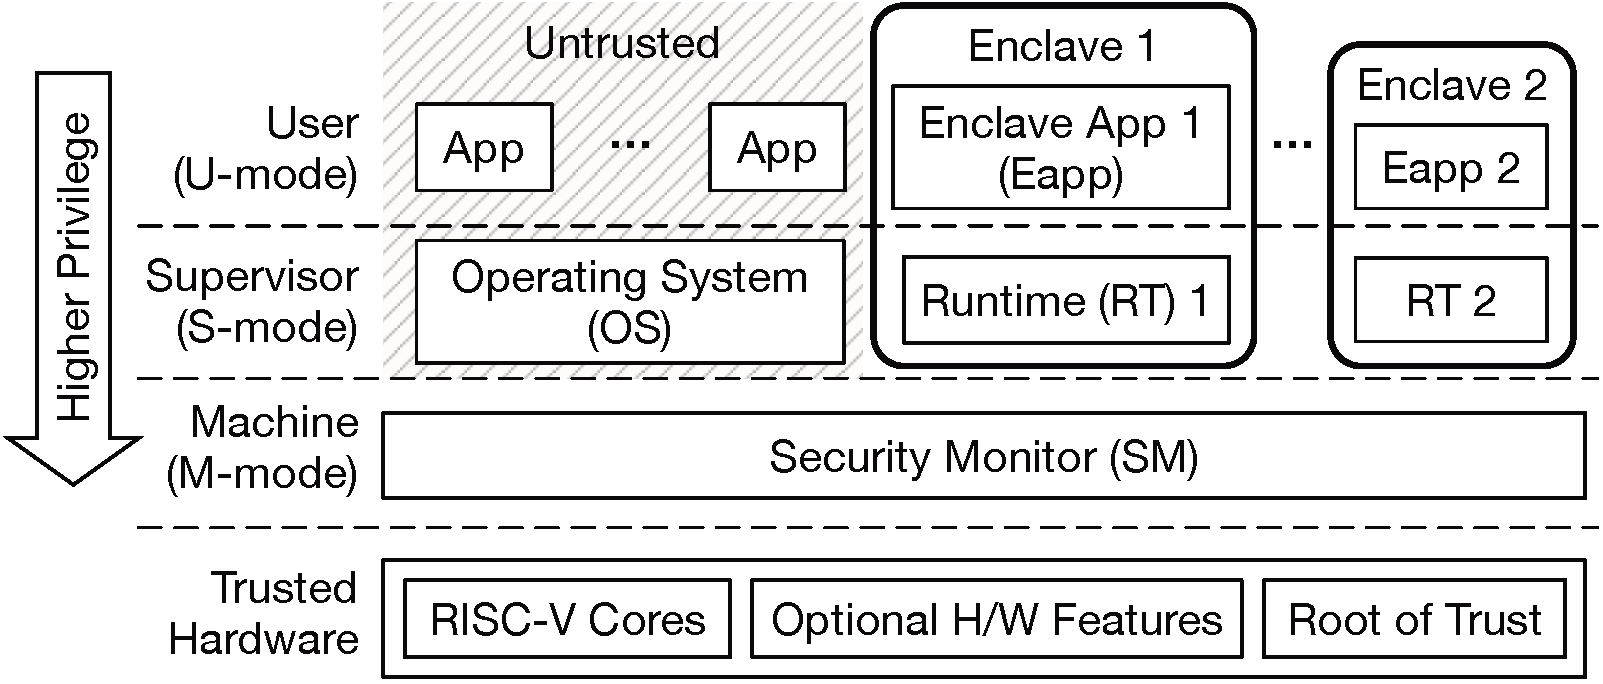
\includegraphics[width=0.9\linewidth]{figures/keystone_overview.png}
    \caption{Overview of the Keystone architecture illustrating components such as the Security Monitor, enclave runtime, and the privilege hierarchy.}
    \label{fig:keystone_overview}
\end{figure}

Enclaves, the fundamental isolation units in Keystone, operate within dedicated physical memory regions inaccessible to the OS and other enclaves. Physical Memory Protection (PMP), a hardware-assisted mechanism controlled by the SM, restricts access to enclave memory exclusively to the enclave and the SM, thus preserving confidentiality and integrity even in the event of OS compromise.

Each enclave comprises two principal layers: the user-level enclave application (eapp) and a supervisor-level runtime environment. The eapp executes user-specific logic within the enclave, while the runtime, operating in supervisor mode (S-mode), manages system calls, exception handling, and virtual memory services intrinsic to enclave operation. This layered design provides a clear separation of concerns, reducing attack surfaces and allowing for customized security policies adapted to workload requirements.

Keystone’s workflow delineates distinct roles for platform providers and enclave developers, fostering modularity and flexibility. Platform providers undertake the compilation and deployment of the SM tailored to the target hardware, ensuring integration of the root of trust and hardware-specific functionalities. Enclave developers leverage the Keystone SDK to construct enclave applications alongside their runtimes and host binaries, which are subsequently packaged and deployed on the target platform independently of underlying hardware specifics.

Furthermore, Keystone supports remote attestation mechanisms, enabling verification of enclave authenticity and integrity prior to provisioning sensitive data or executing critical workloads. This capability is essential for secure deployment in distributed and cloud environments.

The enclave lifecycle progresses through three stages: creation, execution, and destruction. Creation involves the host allocating enclave private memory (EPM), populating it with enclave page tables, runtime, and application binaries, and invoking the SM to isolate the enclave via PMP. During execution, the SM orchestrates transitions into and out of the enclave, dynamically adjusting PMP permissions to maintain strict isolation. Destruction securely clears the enclave’s EPM and reclaims resources, ensuring no residual data remains.

\begin{figure}[htbp]
    \centering
    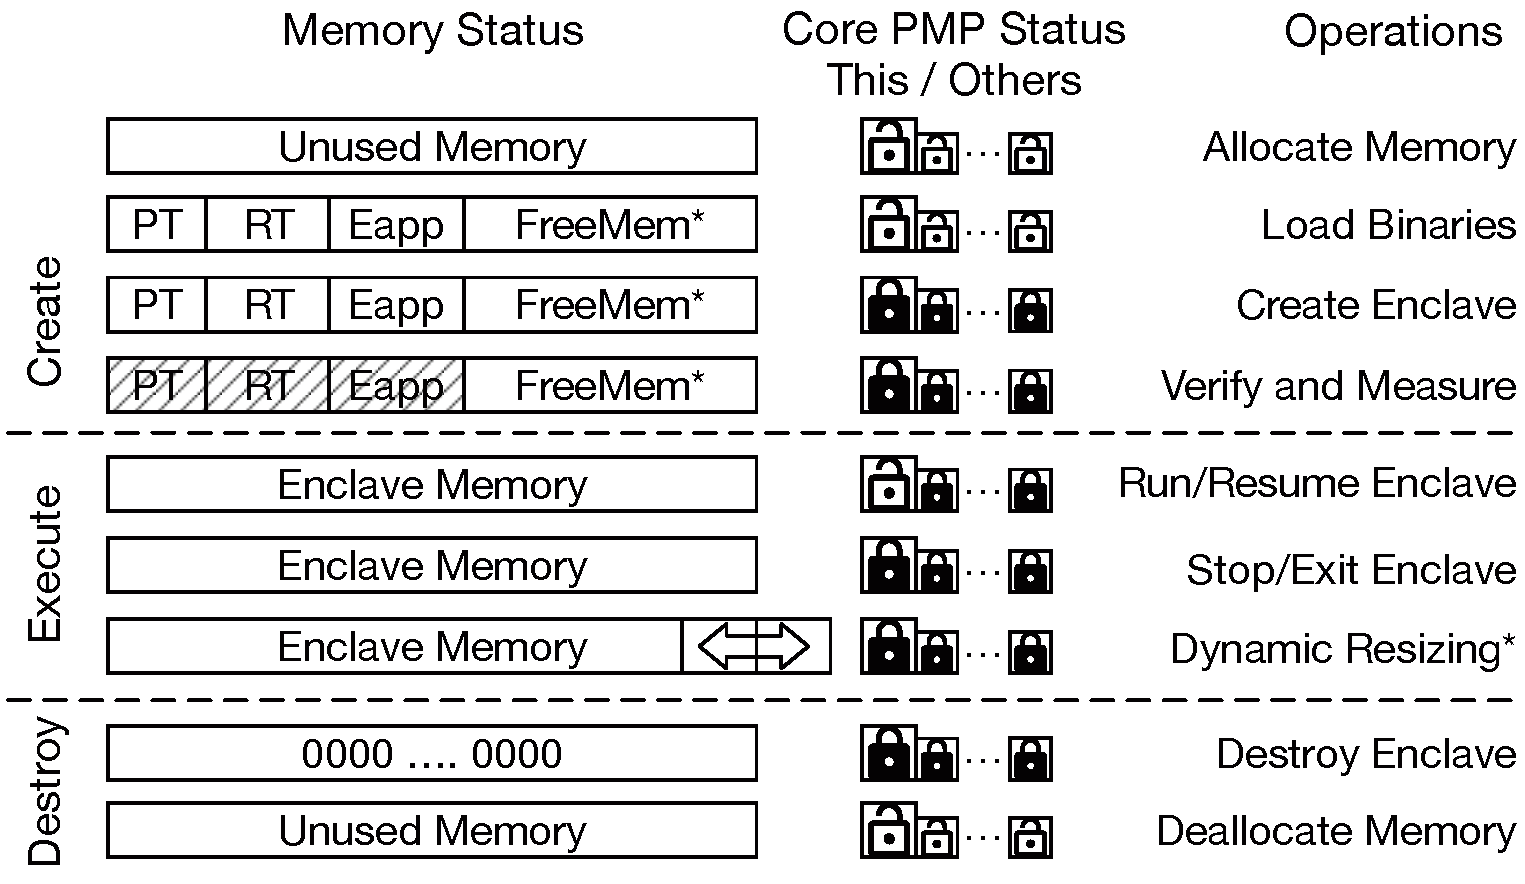
\includegraphics[width=0.9\linewidth]{figures/enclave_lifecycle.png}
    \caption{Stages of a Keystone enclave lifecycle: creation, execution, and destruction.}
    \label{fig:enclave_lifecycle}
\end{figure}

Keystone’s design also facilitates extensibility, allowing for integration of advanced security features such as secure I/O, cryptographic accelerators, and hardware-assisted debugging. This adaptability future-proofs the architecture, enabling continuous evolution of TEE capabilities aligned with emerging threats and diverse application demands on RISC-V platforms.

\section{Comparison with other TEEs}

\section{Performance considerations in TEEs}